\documentclass[aps,prb,reprint,noeprint,superscriptaddress]{revtex4-2}
\pdfoutput=1
\usepackage[utf8]{inputenc}
\usepackage[english]{babel}
\usepackage{microtype}
\usepackage{amsmath,amssymb,amsfonts}
\usepackage{braket}
\usepackage{bm}
\usepackage{graphicx}
\usepackage{booktabs}
\usepackage{comment}

\usepackage{float}
\usepackage[
    pdftitle={},
    pdfauthor={},
    colorlinks=true,
    unicode=true,
    pdfborder={0 0 0},
    allcolors=blue
]{hyperref}

\renewcommand{\vec}[1]{\bm{#1}}
\newcommand{\im}{\mathrm{i}}
\newcommand{\e}{\mathrm{e}}
\renewcommand{\Im}{\operatorname{\mathsf{Im}}}
\renewcommand{\Re}{\operatorname{\mathsf{Re}}}
\newcommand{\vk}{{\vec k}}
\newcommand{\vq}{{\vec q}}
\newcommand{\VV}[2]{\begin{pmatrix}#1\\#2\end{pmatrix}}
\newcommand{\VVT}[2]{\begin{pmatrix}#1 & #2\end{pmatrix}}
\newcommand{\VVV}[3]{\begin{pmatrix}#1\\#2\\#3\end{pmatrix}}
\newcommand{\VVVT}[3]{\begin{pmatrix}#1 & #2 & #3\end{pmatrix}}
\newcommand{\MM}[4]{\begin{pmatrix}#1 & #2 \\ #3 & #4\end{pmatrix}}

\begin{document}

\title{Time-resolved optical conductivity and Higgs oscillations\\in two-band dirty superconductors}

\author{Rafael Haenel}
\affiliation{Max Planck Institute for Solid State Research,
70569 Stuttgart, Germany}
\affiliation{Quantum Matter Institute, University of British Columbia, Vancouver V6T 1Z4, Canada}

\author{Paul Froese}
\affiliation{Max Planck Institute for Solid State Research,
70569 Stuttgart, Germany}
\affiliation{Quantum Matter Institute, University of British Columbia, Vancouver V6T 1Z4, Canada}


\author{Dirk Manske}
\affiliation{Max Planck Institute for Solid State Research,
70569 Stuttgart, Germany}

\author{Lukas Schwarz}
\affiliation{Max Planck Institute for Solid State Research,
70569 Stuttgart, Germany}


\date{\today}

%%%%%%%%%%%%%%%%%%%%%%%%%%%%%%%%%%%%%%%%%%%%%%%%%%%%%%%%
\begin{abstract}
...
\end{abstract}
%%%%%%%%%%%%%%%%%%%%%%%%%%%%%%%%%%%%%%%%%%%%%%%%%%%%%%%%




\maketitle


%%%%%%%%%%%%%%%%%%%%%%%%%%%%%%%%%%%%%%%%%%%%%%%%%%%%%%%%
\section{Introduction}
\label{sec:introduction}
%%%%%%%%%%%%%%%%%%%%%%%%%%%%%%%%%%%%%%%%%%%%%%%%%%%%%%%%

\begin{itemize}
	\item Ultrafast spectroscopy
	\item Collective modes in superconductors: Higgs, Goldstone (shifted to plasma energy due to Anderson-Higgs)
	\item In two-band superconductors: Additional out-of-phase Leggett mode, can couple to Higgs in nonequilibrium
	\item Difficulties excitation Higgs mode, in clean-limit only weak coupling
	\item In dirty superconductors: Coupling is enhanced
	\item This work: 1) Higgs oscillations in two-band sc. with bands in different limits, 2) Nonequilibrium optical conductivity, 3) Leggett mode in dirty-limit, 4) Prediction for MgB$_2$
\end{itemize}







%%%%%%%%%%%%%%%%%%%%%%%%%%%%%%%%%%%%%%%%%%%%%%%%%%%%%%%%
\section{Model}
\label{sec:model}
%%%%%%%%%%%%%%%%%%%%%%%%%%%%%%%%%%%%%%%%%%%%%%%%%%%%%%%%

\begin{itemize}
	\item In this section show only the final formula, all derivation into the appendix A as the equations are similar to the Murotani paper.
	\item Show Hamiltonian, gap equation, Mattis-Bardeen replacement, general approach for calculating time evolution...
	\item I suggest putting the (final) equations for current, optical conductivity, $\delta\Delta(t)$ into the respective section, but in principle we could also put all equations in this section and show only the results in the following sections

	\item Used parameters (take general parameters for section III and IV where no Leggett mode occurs, Leggett mode is discussed later separately and MgB$_2$ will be also discussed later. Show the used parameters in these section)
	\item Implementation details? Are there any subtle points?
\end{itemize}


\begin{eqnarray}
	H_{\text{BCS}} = \sum_{i\mathbf{k}\sigma}  
	\varepsilon_{i\mathbf{k}}c_{i\mathbf{k}\sigma}^\dagger
	c_{i\mathbf{k}\sigma} + \sum_{i\mathbf{k}}^{}
	\left( \Delta_i c_{i\mathbf{-k}\uparrow }^\dagger
	c_{i\mathbf{k}\downarrow }^\dagger  \right) \,,
\end{eqnarray}

where $\varepsilon_{i\mathbf{k}} = s_i \left(\mathbf{k}^2/2m_i -
\varepsilon_{F_i}\right)$ and the superconducting order parameter is self-consistently determined by 
$\Delta_i = \sum_{j\mathbf{k}}^{}U_{ij} \langle c_{j-\mathbf{k}\downarrow
}c_{j\mathbf{k}\uparrow }\rangle$.

\begin{eqnarray*}
	H_{\text{p-p}} = -\sum_{i\mathbf{kk'}\sigma}^{}
	\mathbf{J}_{i\mathbf{kk'}} \cdot \mathbf{A} \,
	c_{i\mathbf{k}\sigma}^\dagger  c_{i\mathbf{k}'\sigma} +
	\sum_{i\mathbf{k}\sigma}^{} \frac{s_i e^2}{2m_i} \mathbf{A}^2 \,
	c_{i\mathbf{k}\sigma}^\dagger c_{i\mathbf{k}\sigma}
\end{eqnarray*}

\begin{eqnarray*}
	\langle \left|\mathbf{e} \cdot
	\mathbf{J}_{i\mathbf{kk'}}\right|^2\rangle_{\text{Av}}
	&=& \int \frac{d\Omega_\mathbf{k}}{4\pi} \frac{d\Omega_\mathbf{k}'}{4\pi}
	\left|\mathbf{e} \cdot \mathbf{J}_{i\mathbf{kk'}}\right|^2
	\\
	&\approx& \frac{(e v_{F_i})^2}{3 \pi N_i(0)} 
	\frac{\gamma_i}{(\varepsilon-\varepsilon')^2 + \gamma_i^2}
\end{eqnarray*}

Discussion of $A, A^2$.

The full Hamiltonian is given by $H = H_{BCS} + H_{p-p}$.






\section{Single-band superconductivity}

\begin{figure}[ht]
	\centering
	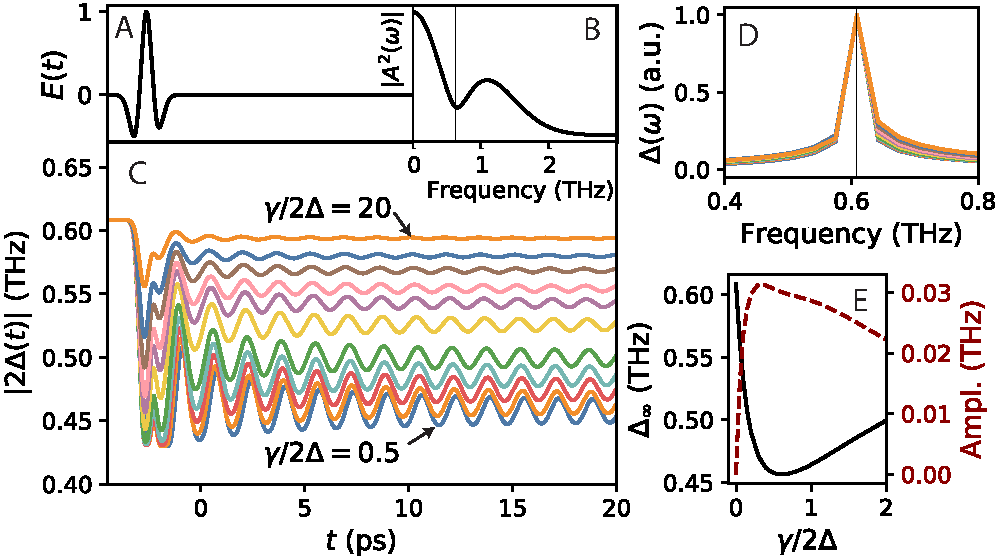
\includegraphics[width=\columnwidth]{figures/fig1.pdf}
	\caption{ABC}
\end{figure}

\begin{figure}[ht]
	\centering
	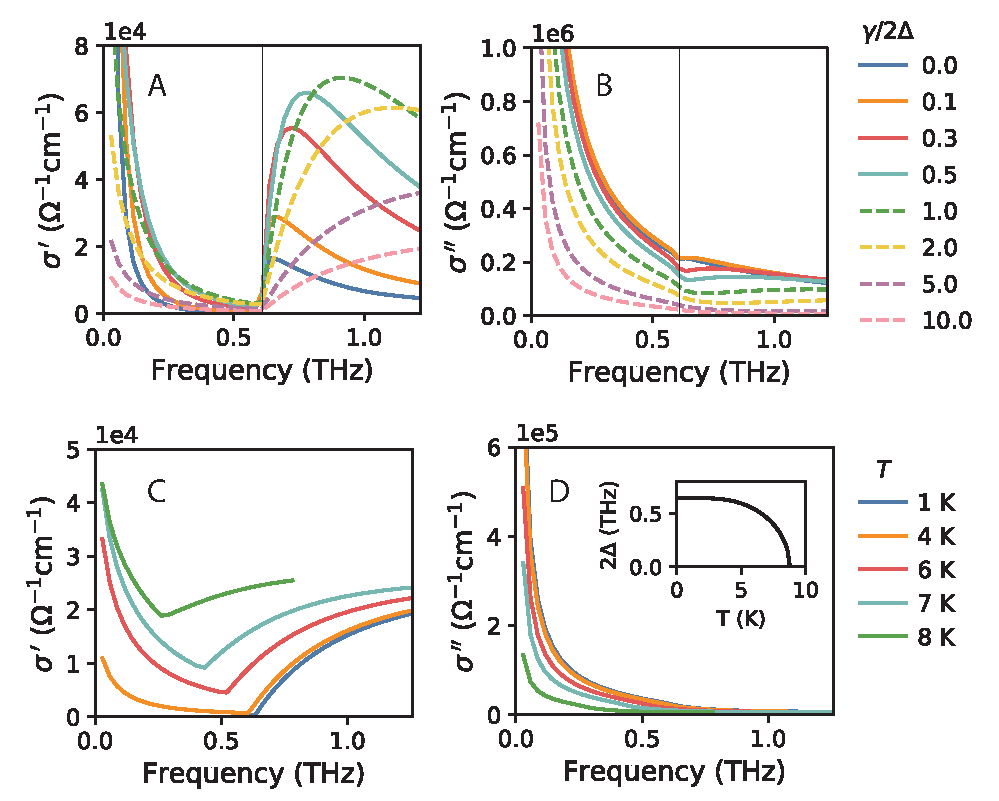
\includegraphics[width=\columnwidth]{figures/fig2.pdf}
	\caption{ABC}
\end{figure}

\begin{figure}[ht]
	\centering
	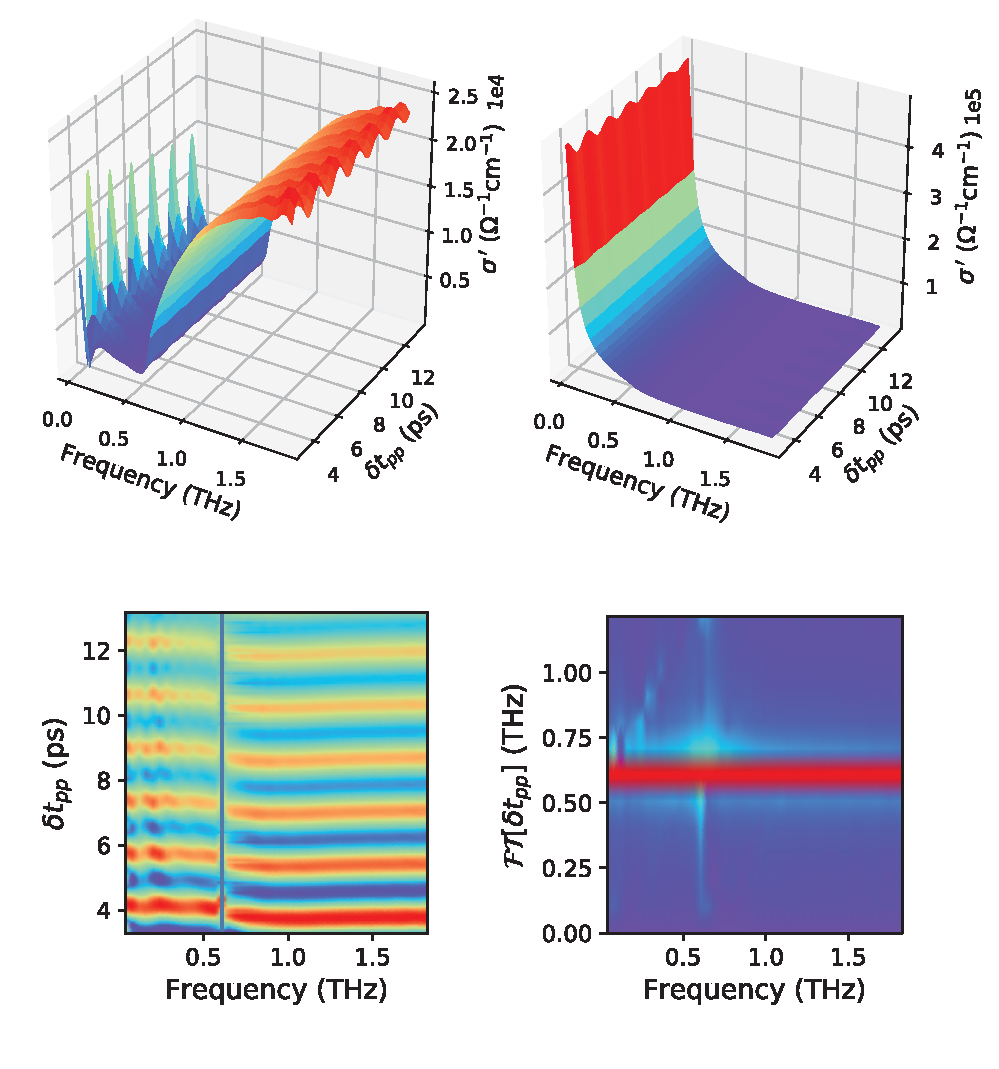
\includegraphics[width=\columnwidth]{figures/fig3.pdf}
	\caption{ABC}
\end{figure}
%\begin{comment}
%%%%%%%%%%%%%%%%%%%%%%%%%%%%%%%%%%%%%%%%%%%%%%%%%%%%%%%%
\section{Higgs oscillations}
\label{sec:higgs_oscillations}
%%%%%%%%%%%%%%%%%%%%%%%%%%%%%%%%%%%%%%%%%%%%%%%%%%%%%%%%

\begin{itemize}
	\item Equation for Current
	\item Equation for optical conductivity
	\item Present and discuss equilibrium optical conductivity in Fig. 1 for the four different limit cases, used in the rest of the paper
\end{itemize}


\begin{figure}[H]
    \centering
    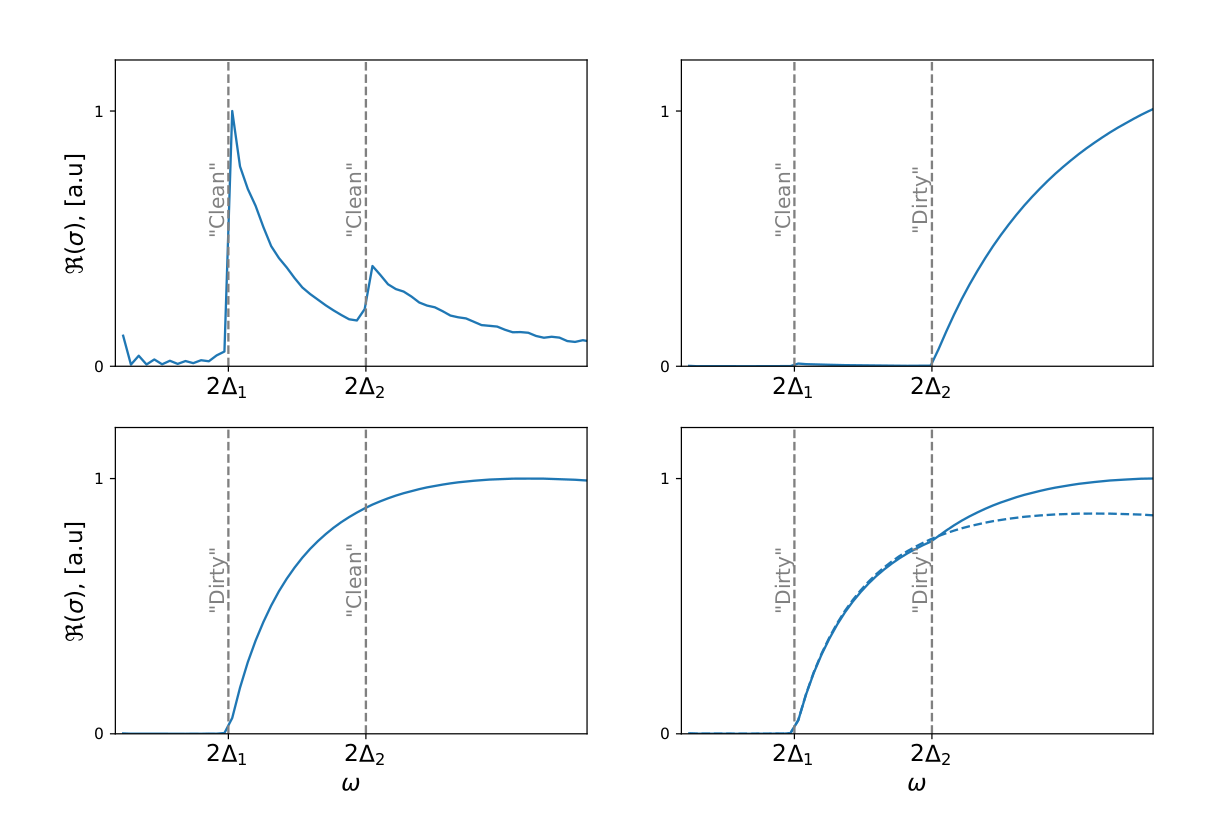
\includegraphics[width=\columnwidth]{figures/two_band_cond.png}
    \caption{\label{fig:two_band_cond}%
    Equilibrium optical conductivity of a two-band superconductor with gaps in different impurity scattering limits (clean-clean case rescaled as response is much smaller?)}
\end{figure}%

\begin{itemize}
	\item Equation for $\delta\Delta(t)$
	\item Show and discuss Higgs oscillations in Fig. 2 of the four cases with a suitable pump pulse (refer to appendix B for details about the pump pulse)
\end{itemize}

\begin{figure}[H]
    \centering
    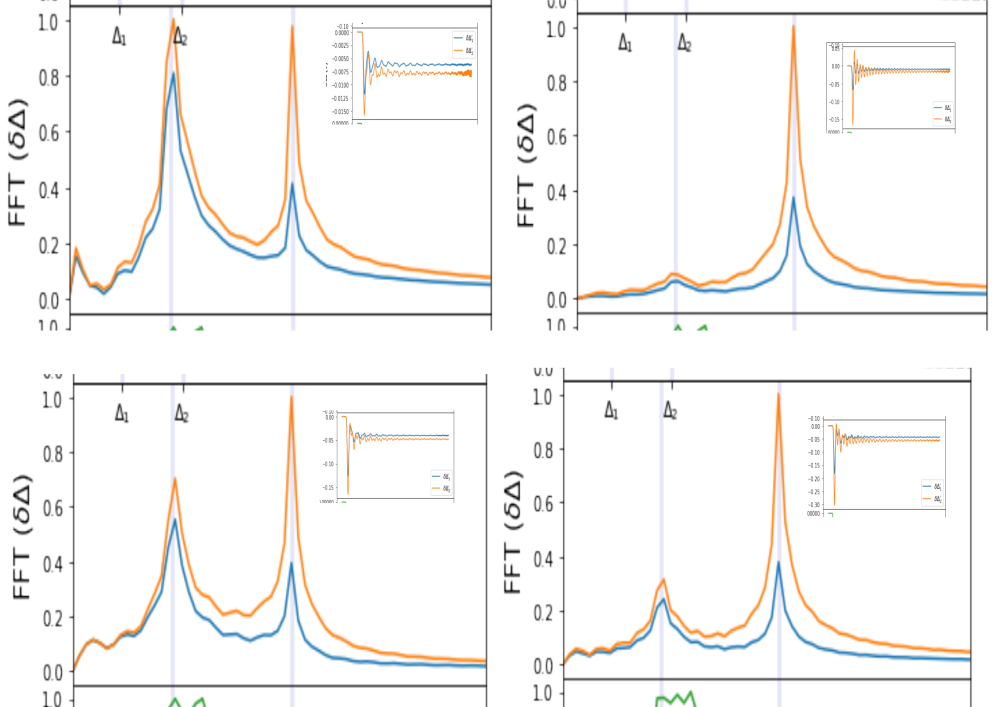
\includegraphics[width=\columnwidth]{figures/gap_osci.png}
    \caption{\label{fig:gap_osci}%
    Higgs oscillations excited by a pump pulse with enough bandwidth to cover both gaps for the different impurity scattering limits shown in Fig.~\ref{fig:two_band_cond}}
\end{figure}%








%%%%%%%%%%%%%%%%%%%%%%%%%%%%%%%%%%%%%%%%%%%%%%%%%%%%%%%%
\section{Nonequilibrium optical conductivity}
\label{sec:noneq_cond}
%%%%%%%%%%%%%%%%%%%%%%%%%%%%%%%%%%%%%%%%%%%%%%%%%%%%%%%%

\begin{itemize}
	\item Equation for nonequilibrium optical conductivity with two pulses. Maybe here more details (instead of appendix), as this is not covered by the Murotani paper
	\item Show and discuss nonequlibrium conductivity in Fig. 3.
	\item More figures of nonequilibrium conductivity? Suggestions: Imaginary part, maybe appendix. Nice 3d plot. Oscillations along cuts.
\end{itemize}


\begin{figure}[H]
    \centering
    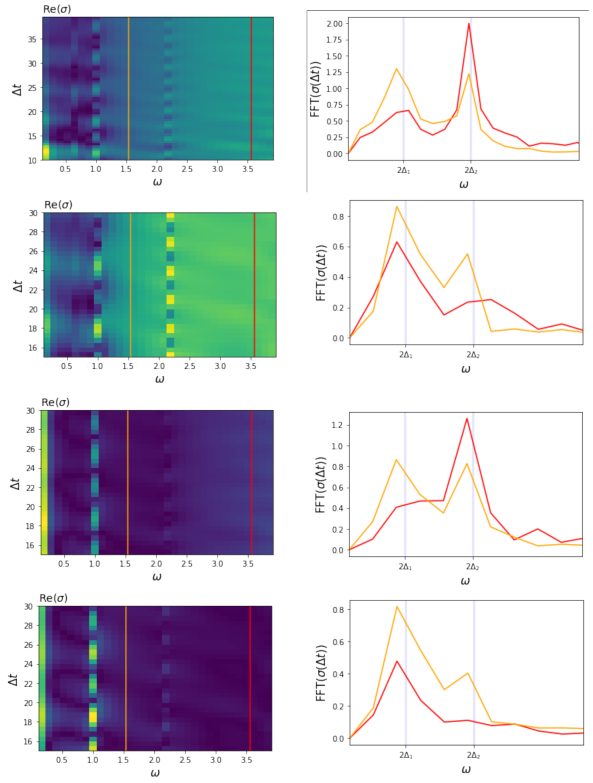
\includegraphics[width=\columnwidth]{figures/noneq_cond.png}
    \caption{\label{fig:noneq_cond}%
    Nonequilibrium optical conductivity of a pump-probe experiment for the different impurity scattering limits shown in Fig.~\ref{fig:two_band_cond}}
\end{figure}%


%%%%%%%%%%%%%%%%%%%%%%%%%%%%%%%%%%%%%%%%%%%%%%%%%%%%%%%%
\section{Leggett mode}
\label{sec:leggett_mode}
%%%%%%%%%%%%%%%%%%%%%%%%%%%%%%%%%%%%%%%%%%%%%%%%%%%%%%%%

\begin{itemize}
	\item Definition, equation of Leggett mode
	\item Parameters for Fig.4 where Leggett mode occurs
	\item Discuss Fig. 4
	\item Maybe rethink what exactly to show in Fig. 4
	\item New plot of time-resolved conductivity showing Leggett mode?
\end{itemize}

\begin{figure}[H]
    \centering
    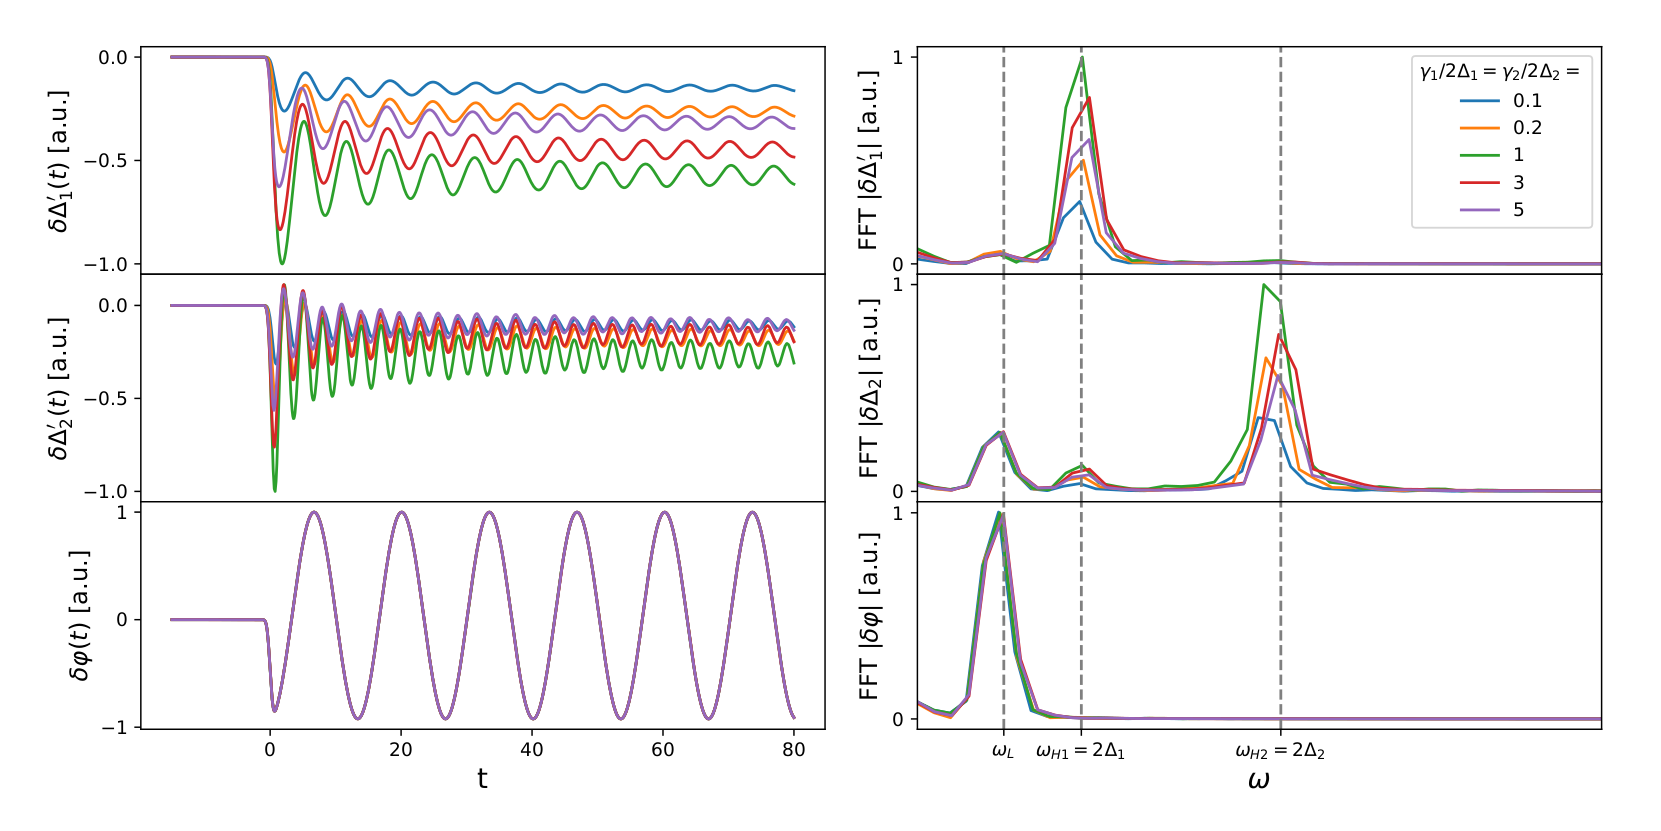
\includegraphics[width=\columnwidth]{figures/leggett_oscillations.png}
    \caption{\label{fig:leggett_oscillations}%
    Induced amplitude (Higgs) and out-of-phase (Leggett) oscillations of a two-band superconductor for different impurity scattering rates}
\end{figure}%

\begin{itemize}
	\item Discuss Fig. 5 for varying coupling strength and compare with clean limit result
\end{itemize}

\begin{figure}[H]
    \centering
    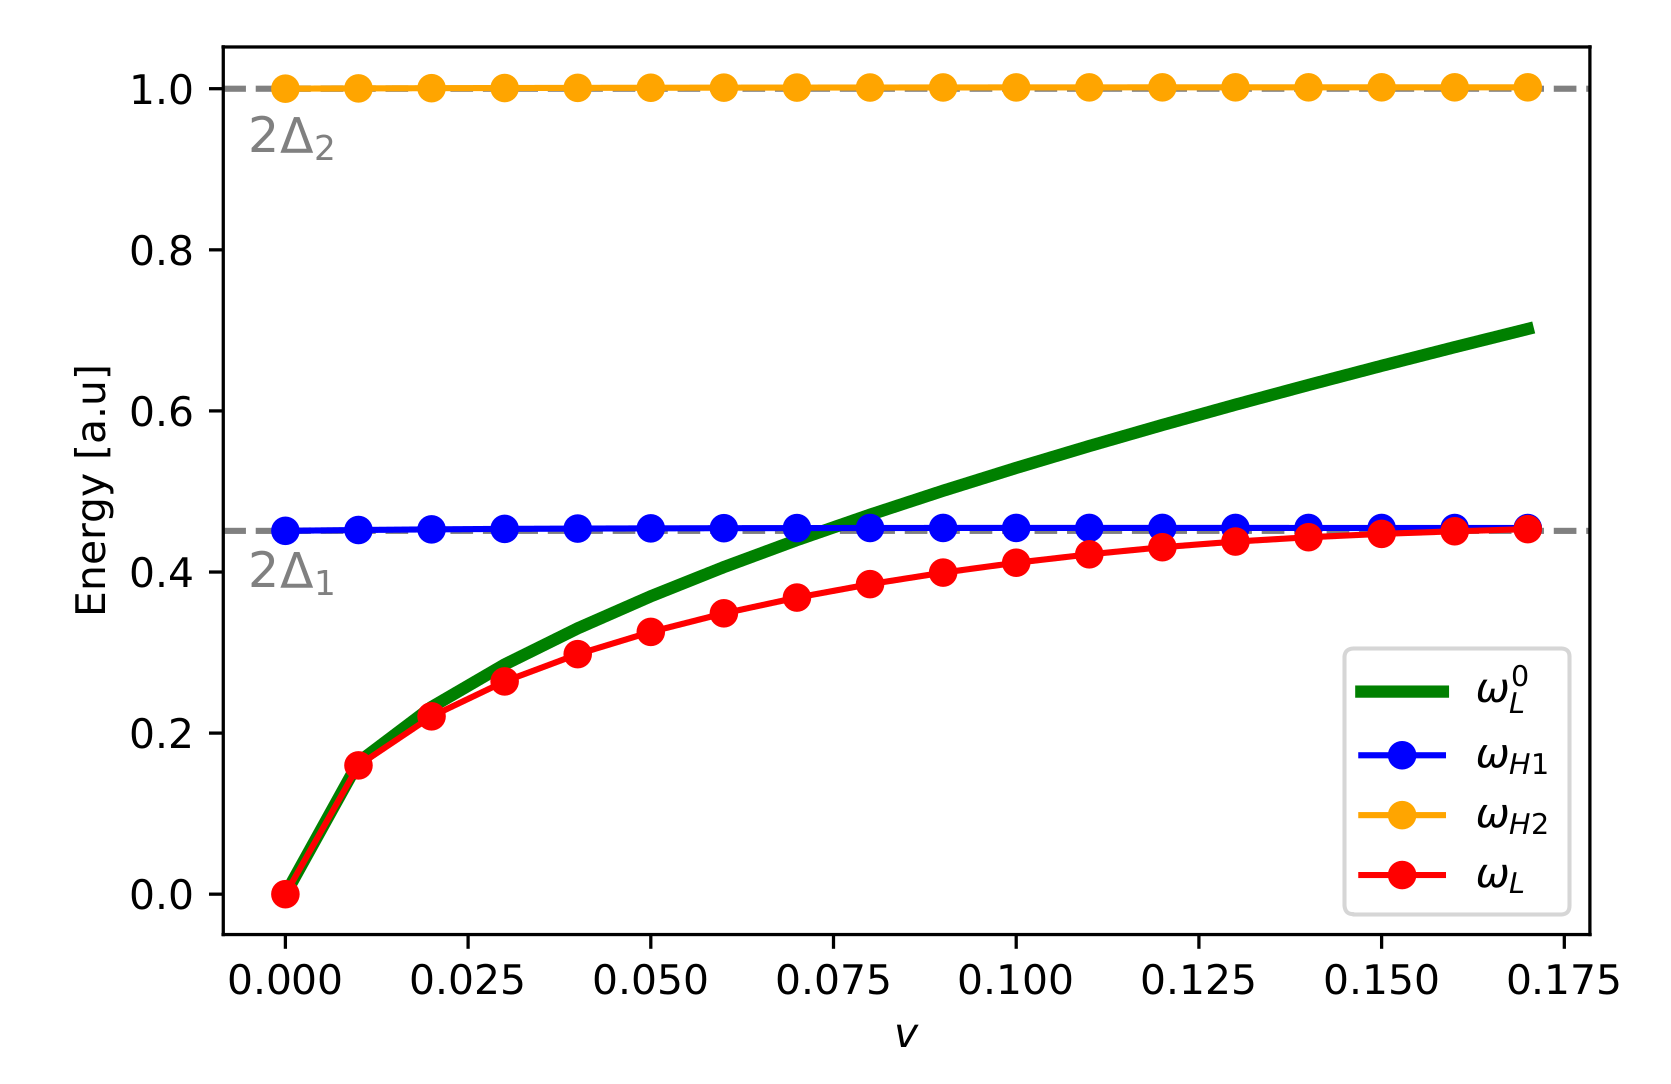
\includegraphics[width=\columnwidth]{figures/leggett_coupling.png}
    \caption{\label{fig:leggett_coupling}%
    Frequency of Leggett mode as function of interband coupling strength in the dirty limit}
\end{figure}%



%%%%%%%%%%%%%%%%%%%%%%%%%%%%%%%%%%%%%%%%%%%%%%%%%%%%%%%%
\section{MgB$_2$}
\label{sec:mgb2}
%%%%%%%%%%%%%%%%%%%%%%%%%%%%%%%%%%%%%%%%%%%%%%%%%%%%%%%%

\begin{itemize}
	\item Parameters which match MgB$_s$
	\item Show prediction in Fig. 6 of equilibrium conductivity, Higgs oscillations, nonequilibrium conductivity
\end{itemize}

\begin{figure}[H]
    \centering
    %\includegraphics[width=\columnwidth]{figures/mgb2.png}
    \Huge{TODO}
    \caption{\label{fig:mgb2}%
    Result with parameters for MgB$_2$ a) Equilibrium optical conductivity, b) Higgs oscillations, c) pump-probe conductivity and spectra}
\end{figure}%



%%%%%%%%%%%%%%%%%%%%%%%%%%%%%%%%%%%%%%%%%%%%%%%%%%%%%%%%
\section{Conclusion}
\label{sec:conclusion}
%%%%%%%%%%%%%%%%%%%%%%%%%%%%%%%%%%%%%%%%%%%%%%%%%%%%%%%%

...







%%%%%%%%%%%%%%%%%%%%%%%%%%%%%%%%%%%%%%%%%%%%%%%%%%%%%%%%
\begin{acknowledgments}
...
\end{acknowledgments}
%%%%%%%%%%%%%%%%%%%%%%%%%%%%%%%%%%%%%%%%%%%%%%%%%%%%%%%%






%%%%%%%%%%%%%%%%%%%%%%%%%%%%%%%%%%%%%%%%%%%%%%%%%%%%%%%%
\bibliography{literature}
%%%%%%%%%%%%%%%%%%%%%%%%%%%%%%%%%%%%%%%%%%%%%%%%%%%%%%%%




%%%%%%%%%%%%%%%%%%%%%%%%%%%%%%%%%%%%%%%%%%%%%%%%%%%%%%%%
%\end{comment}
\appendix
%%%%%%%%%%%%%%%%%%%%%%%%%%%%%%%%%%%%%%%%%%%%%%%%%%%%%%%%


%%%%%%%%%%%%%%%%%%%%%%%%%%%%%%%%%%%%%%%%%%%%%%%%%%%%%%%%
\section{Derivation of nonequilibrium optical conductivity}
\label{sec:derivation_noneq_cond}
%%%%%%%%%%%%%%%%%%%%%%%%%%%%%%%%%%%%%%%%%%%%%%%%%%%%%%%%


\begin{itemize}
	\item Put here all equations and derivations of the main results
\end{itemize}






%%%%%%%%%%%%%%%%%%%%%%%%%%%%%%%%%%%%%%%%%%%%%%%%%%%%%%%%
\section{Influence of pump pulse frequency}
\label{sec:influence_pump_pulse_freq}
%%%%%%%%%%%%%%%%%%%%%%%%%%%%%%%%%%%%%%%%%%%%%%%%%%%%%%%%

\begin{itemize}
	\item Discuss influence of pump pulse frequency and bandwith to excite only one or both Higgs mode
	\item Show result in Fig. 7
\end{itemize}

\begin{figure}[H]
    \centering
    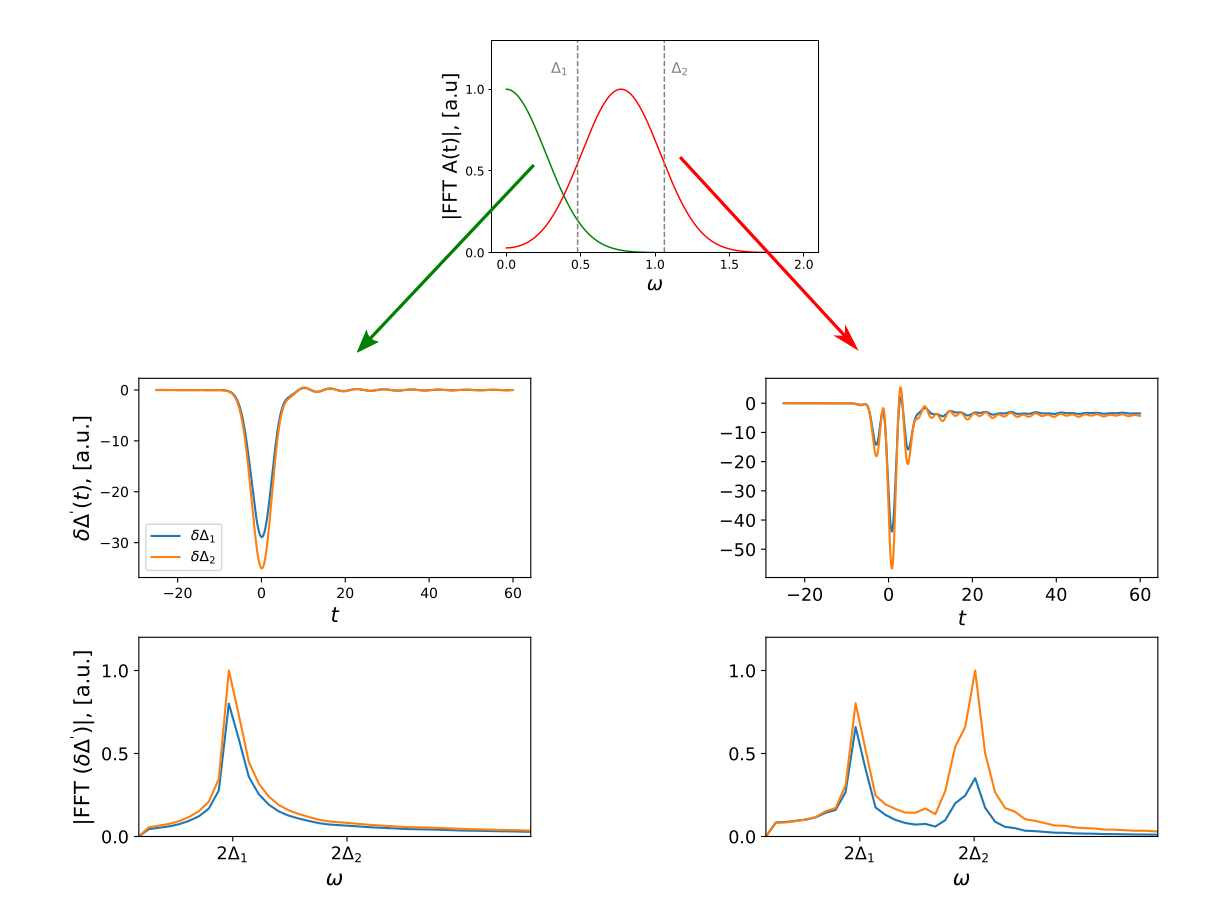
\includegraphics[width=\columnwidth]{figures/influence_pump_pulse_freq.png}
    \caption{\label{fig:influence_pump_pulse_freq}%
    Influence of pump pulse frequency}
\end{figure}%



\end{document}
